Invariants are all derived from one common class \class{Invariant}, see figure \ref{fig_invariant}, such that they 
all implement the same methods. This is very useful when doing local search. 
\begin{figure}[!b]
\begin{center}
 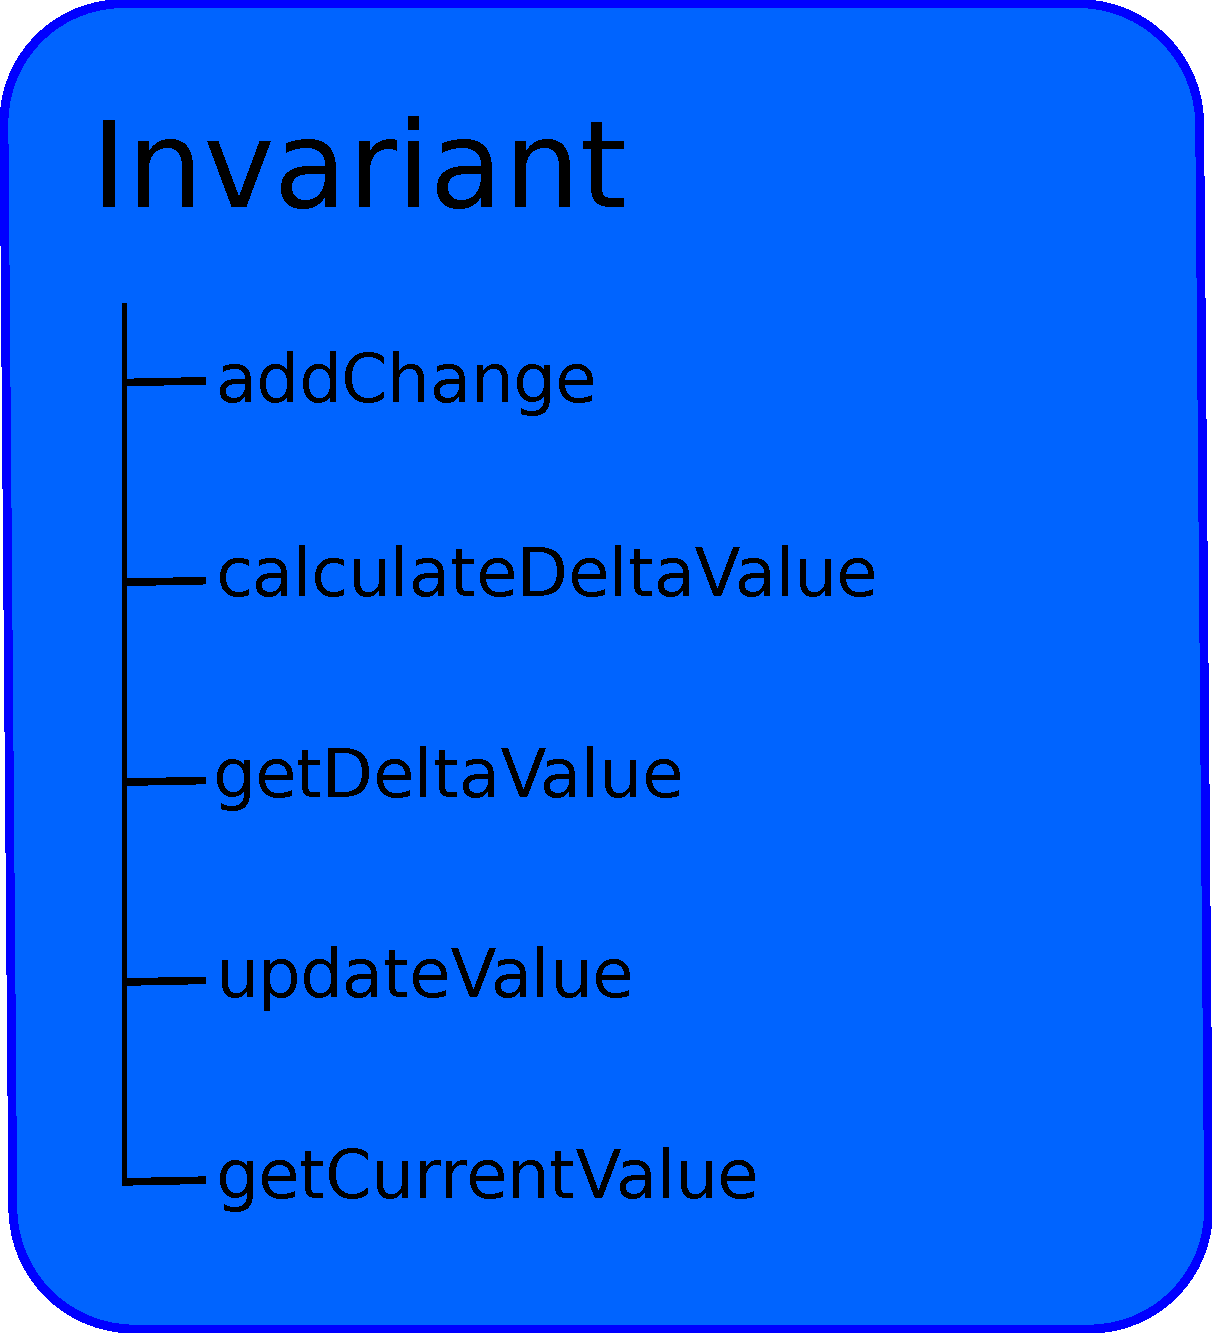
\includegraphics[width=\linewidth/2]{invariant.pdf} \caption{Important methods in Invariant 
class.}\label{fig_invariant}
\end{center} 
\end{figure}
Invariants are only introduced after an initial solution to an instance has been found and before the local 
search has begun. Invariants can represent either a variable or an auxiliary variable and are defined by oneway 
constraints. The invariants classes that are implemented contain information about how the invariant is defined and the 
value of the invariant. Hence the \class{invariant} classes are representing both the oneway constraint and the 
invariant. \\ 
All subclasses of \class{Invariant} have a delta value, a current value, coefficient map, a stack of changes, a lower 
bound, and an upper bound. These are used by the different methods of the invariants. \\
All Invariants must implement the methods \method{proposeChange}, \method{calculateDelta}, and 
\method{updateValue} which are used during local search. When suggesting a new 
value to a variable the method \method{proposeChange} is used. The proposed change is put on the stack until the 
the method \method{calculateDelta} is called. \method{calculateDelta} is used by the delta evaluation function in local 
search and updates the delta value of the invariant according to the changes received from \method{proposeChange}. The 
method \method{updateValue} is called when a neighborhood operation is commited, to update the value of the invariant. 
\\ Each type of invariant must implement its own method since the methods can be different for each type of invariant. 
\\ 
Different classes use the invariants but do not differentiate between them since they all have the same methods.  
If invariants did not have a common super class then each invariant type would need its own data structure for 
storage. Another benefit is the search procedures do not have to examine which invariants the model consist of since 
they all have the same methods. It also makes it easier to add new invariants since all the functionality are 
implemented by the new invariant and nothing has to be changed in the \class{LocalSearchEngine}. \\ 
\subsubsection{Implementation of Sum}
The class \class{Sum} is used to define variables or auxiliary variables by a summation of variables multiplied by 
their coefficient with a constant offset. I.e. $x_1 = 2x_2+4x_3 + 1$, \class{Sum} can represent the right hand side in 
the equation defining $x_1$. \\ 
The method \method{proposeChange}(int  $variableID$, int $valueChange$) uses the variables id to 
get its coefficient from a hashmap. The coefficient multiplied by the integer $valueChange$, the change of the 
variables value, gives the delta value that is pushed on a stack $variableChange$. \\ 
The method \method{calculateDelta}() first resets the delta value to zero and then pop each integer on the stack 
and add them to the delta value. The implementation can be seen in algorithm \ref{algo_calcDelta}. 

\IncMargin{1em}
\begin{algorithm}[H]

%\SetKwFunction{relation}{relation}\SetKwFunction{coeff}{coefficient}
  \algdata
\Input{stack VariableChange}
\Output{\bool allowed}
%\BlankLine
    \int $DeltaValue$ = 0 \;
    \While{VariableChange $\neq \emptyset$}{
        $DeltaValue$ += VariableChange.pop()\;
    }
    \uIf{$DeltaValue + CurrentValue < lowerbound$} {
        \Return \false\;
    }\uElseIf{$DeltaValue + CurrentValue > upperbound$}{ 
  \Return \false \;
    }\Else{
    \Return \true \;
    }
\caption{Sum - calculateDelta()} \label{algo_calcDelta} 
 %\caption{Test if a constraint $c$ can define a variable $x$ } \label{algo_checkoneway}
\end{algorithm} \noindent
\DecMargin{1em} \\
It checks if the new value would violated the bounds of the \class{Invariant} in case it is used to define a variable. 
By returning false it tells the new value would not be within the bounds of the invariant hence the change cannot be 
allowed. This will 
be used during local search in section \ref{sec_local}. \\
It updates its value by adding the delta value to the current value in the method \method{updateValue()}.

\subsubsection{Implementation of LEQViolation and EQViolation}
The invariant \class{LEQViolation} and \class{LEQViolation} are used for measuring violation of a constraint. They are
relations between the value of an invariant and an integer. The value of \class{LEQViolation} is zero if and only if 
the value of the invariant is less than the integer. The value is the difference between the invariants value and the 
integer otherwise. For \class{LEQViolation} the value is zero if they are equal otherwise the absolute value of 
the difference. \\ 
\method{proposeChange} and \method{updateValue} are implemented almost same as in \class{Sum} but 
\method{proposeChange} does not use the coefficient hashmap. \\ 
Algorithm \ref{algo_calcDelta2} and \ref{algo_calcDelta3} is the implementation of \method{calculateDelta}. \\ 
\IncMargin{1em}
\begin{algorithm}[H]

%\SetKwFunction{relation}{relation}\SetKwFunction{coeff}{coefficient}
  \algdata
\Input{stack VariableChange, \int LHS}
\Output{\bool allowed}
\BlankLine
    \If{VariableChange $= \emptyset$}{
      $DeltaValue$ = 0 \;
      \Return \true\;
    }
    \eIf{LHS + VariableChange.pop() $\leq$ RHS} {
    $DeltaValue = -CurrentValue $\;
    }{
      \int $old = max(LHS-RHS,0) $\;
      \int $new = max(LHS+VariableChange.pop() - RHS,0) $\;
      $DelataValue = new-old $\;
    }
    \Return \true \;
\caption{LEQViolation - calculateDelta()} \label{algo_calcDelta2} 
 %\caption{Test if a constraint $c$ can define a variable $x$ } \label{algo_checkoneway}
\end{algorithm} \noindent
\DecMargin{1em} \\

\IncMargin{1em}
\begin{algorithm}[H]

%\SetKwFunction{relation}{relation}\SetKwFunction{coeff}{coefficient}
  \algdata
\Input{stack VariableChange, \int LHS}
\Output{\bool allowed}
\BlankLine
    \If{VariableChange $= \emptyset$}{
      $DeltaValue$ = 0 \;
      \Return \true\;
    }
    \eIf{LHS + VariableChange.pop() $\leq$ RHS} {
    $DeltaValue = -CurrentValue $\;
    }{
      \int $old = max(LHS-RHS,0) $\;
      \int $new = max(LHS+VariableChange.pop() - RHS,0) $\;
      $DelataValue = new-old $\;
    }
    \Return \true \;
\caption{EQViolation - calculateDelta()} \label{algo_calcDelta3} 
 %\caption{Test if a constraint $c$ can define a variable $x$ } \label{algo_checkoneway}
\end{algorithm} \noindent
\DecMargin{1em} 
The bounds of these invariants are always satisfied. 

